A simulação da placa analógica (Seção~\ref{sec:spice}) usa um modelo comportamental do DAC0800 escrito pelo autor e mantido no repositório LTSpice-behavioral-IC-lib \cite{seifert2026spice}. Esse repositório reúne modelos SPICE de circuitos integrados e apoia o kit educacional de LTspice da \acs{utfpr}, câmpus Campo Mourão. O modelo não descreve os transistores do circuito integrado: cada bloco do diagrama da folha de dados \cite{ti2013} é reproduzido pelo seu comportamento nos terminais, com os valores típicos da tabela de características elétricas e das curvas. O objetivo é simular o conversor como parte de um circuito, com rapidez e boa convergência, sem perder as especificações que importam no projeto.

\section{Estrutura do modelo}

O modelo é um único subcircuito, \cod{DAC0800}, com os 16 terminais na ordem dos pinos do encapsulamento DIP. A Figura~\ref{fig:modelo_dac0800} mostra os seus dois caminhos. No de cima, a referência define a corrente de escala completa. No de baixo, os oito bits decidem que fração dessa corrente vai para cada saída.

\begin{figure}
	\caption{Blocos do modelo comportamental do DAC0800.}
	\label{fig:modelo_dac0800}
	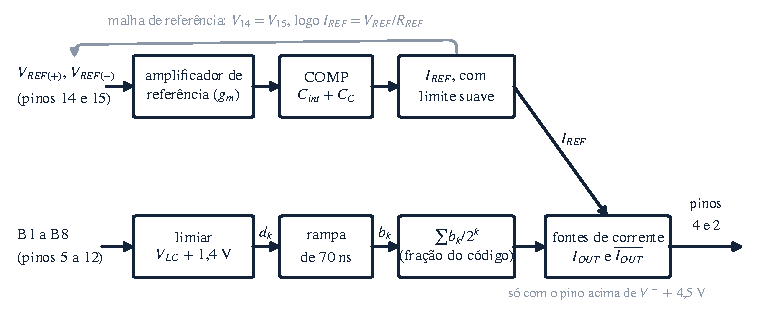
\includegraphics[width=\textwidth]{./figuras/modelo_dac0800}
	\legend{Fonte~---~Autoria própria.}
\end{figure}

\begin{description}
	\item[Amplificador de referência] --- um estágio de transcondutância injeta no nó COMP a corrente \(I_{1,max} \tanh\!\left[g_{m1} (V_{14} - V_{15}) / I_{1,max}\right]\), com \(g_{m1} = 0{,}4\)~mS e \(I_{1,max} = 40~\mu\)A. Esse limite de corrente, carregando a capacitância de COMP, reproduz a taxa de variação de 8~mA/\(\mu\)s da folha de dados. O nó COMP tem 5~pF internos, aos quais se soma o capacitor de compensação externo \(C_C\);
	\item[Corrente de referência] --- a tensão em COMP define a corrente drenada pelo pino 14, \(I_{lin} = g_{m2} (V_{COMP} - V^- - 1{,}4~\text{V})\), com \(g_{m2} = 1\)~mA/V. Como essa corrente passa pelo resistor de referência externo, a malha força \(V_{14} = V_{15}\), e a corrente se acomoda em \(V_{REF}/R_{REF}\), como no circuito real. A corrente é limitada de forma suave, \(I_{REF} = I_{lin} / [1 + (I_{lin}/I_{max})^8]^{1/8}\), em \(I_{max}\) entre 2,1~mA, com \(V^- = -5\)~V, e 4,2~mA, com \(V^- \le -8\)~V, a faixa da folha de dados. Ela também se anula quando o pino 15 fica a menos de 4,5~V de \(V^-\);
	\item[Entradas lógicas] --- cada bit é convertido em um valor \(d_k\) entre 0 e 1 por uma rampa linear de \(\pm 0{,}1\)~V em torno do limiar \(V_{LC} + 1{,}4\)~V. Uma entrada em nível baixo fornece 2~\(\mu\)A para fora do pino, e cada entrada tem 2~pF;
	\item[Comutação] --- o valor efetivo de cada bit, \(b_k\), segue \(d_k\) com inclinação limitada: a transição completa leva 70~ns, com 35~ns até a metade, como os tempos de propagação típicos. A rampa é escrita como \(b_k = d_k - y_k\), em que \(y_k\) é a tensão de um capacitor descarregado por uma corrente constante. Em regime permanente, \(y_k = 0\), e o ponto de operação não exige nenhuma busca;
	\item[Saídas] --- as duas saídas drenam corrente, conforme a Equação~(\ref{eq:modelo_saidas}), com a corrente residual \(I_{ZS} = 0{,}2~\mu\)A em cada uma. Cada saída só conduz enquanto o pino está pelo menos 4,5~V acima de \(V^-\), o limite de conformidade de \(-10{,}5\)~V com alimentação de \(\pm15\)~V. Cada saída tem ainda 5~pF e 1~G\(\Omega\) para \(V^-\);
	\item[Alimentação] --- a corrente de \(V^+\) para \(V^-\) é \(2{,}2~\text{mA} + 10~\mu\text{A/V} \cdot (V^+ - V^-)\). As correntes de referência e de saída retornam por \(V^-\), como no componente.
\end{description}

\begin{equation}\label{eq:modelo_saidas}
	I_{OUT} = I_{REF} \sum_{k=1}^{8} \frac{b_k}{2^k} + I_{ZS},
	\qquad
	\overline{I_{OUT}} = I_{REF} \left(\frac{255}{256} - \sum_{k=1}^{8} \frac{b_k}{2^k}\right) + I_{ZS}.
\end{equation}

Todos os elementos que saturam mantêm uma inclinação de 0,1\% fora da faixa útil. Assim, o método de Newton do simulador sempre encontra uma direção para convergir. Nenhuma fonte depende explicitamente do tempo, o que permite também análises de pequenos sinais.

\section{Parâmetros}

Os valores típicos da folha de dados são os padrões, e qualquer um pode ser alterado na instância do subcircuito (Tabela~\ref{tab:modelo_dac0800}).

\begin{table}
	\caption{Parâmetros do modelo do DAC0800.}
	\label{tab:modelo_dac0800}
	\begin{tabular}{p{0.24\textwidth} p{0.2\textwidth} p{0.46\textwidth}}\toprule
		Parâmetro & Padrão & Significado\\\midrule
		\cod{VTHO}, \cod{VTHW} & 1,4~V; 0,1~V & limiar lógico acima de \(V_{LC}\); meia largura da transição\\
		\cod{TSW} & 70~ns & duração da rampa de comutação de um bit\\
		\cod{IIL}, \cod{CIN} & 2~\(\mu\)A; 2~pF & corrente de uma entrada em nível baixo; capacitância de entrada\\
		\cod{IZS} & 0,2~\(\mu\)A & corrente residual de cada saída\\
		\cod{COUT} & 5~pF & capacitância de cada saída\\
		\cod{GM1}, \cod{I1MAX}, \cod{CINT} & 0,4~mS; 40~\(\mu\)A; 5~pF & amplificador de referência: transcondutância, limite de corrente e compensação interna\\
		\cod{GM2} & 1~mA/V & corrente de referência por volt em COMP\\
		\cod{VCMN} & 4,5~V & limite de conformidade e de modo comum acima de \(V^-\)\\
		\cod{IBREF} & 1~\(\mu\)A & corrente de polarização que sai do pino 15\\\bottomrule
	\end{tabular}
	\legend{Fonte~---~Autoria própria.}
\end{table}

\section{Uso na simulação deste trabalho}

No esquemático da Figura~\ref{fig:ltspice}, o DAC0800 é a instância U1, com todos os parâmetros nos valores padrão. O pino \(V_{LC}\) está no terra, o que põe o limiar lógico em 1,4~V, compatível com os níveis de 3,3~V do \ac{fpga}. A referência de +10~V chega ao pino 14 por um resistor de 5~k\(\Omega\), e o pino 15 vai ao terra por outro de 5~k\(\Omega\), os mesmos R1 e R2 da placa. Isso dá \(I_{REF} = 2\)~mA. O capacitor de compensação é de 100~nF, ligado a \(V^-\). Com esse valor, a malha de referência fica lenta e silenciosa, o que é adequado a uma referência fixa. As duas saídas alimentam o conversor corrente-tensão diferencial.

\section{Verificação}

O repositório de origem tem uma suíte de 34 verificações, executadas no simulador ngspice, que comparam o modelo com as tabelas e as curvas da folha de dados. Todas passam. A Tabela~\ref{tab:verificacao_dac0800} reúne as principais.

\begin{table}
	\caption{Principais verificações do modelo do DAC0800, com \(\pm15\)~V, \(V_{REF} = 10\)~V e \(R_{REF} = 5\)~k\(\Omega\).}
	\label{tab:verificacao_dac0800}
	\begin{tabular}{p{0.38\textwidth} p{0.25\textwidth} p{0.25\textwidth}}\toprule
		Grandeza & Modelo & Folha de dados\\\midrule
		Os 256 códigos & monotônicos, maior desvio de 0,13~\acs{lsb} & monotônico, não linearidade de até 0,19\% da escala\\
		Sete códigos da Tabela 1 da folha de dados (saída unipolar) & a menos de 1/2~\acs{lsb} & valores tabelados\\
		Limiar lógico com \(V_{LC} = 0\) & 1,40~V & \(V_{LC} + 1{,}4\)~V\\
		Tempo de propagação & 35,6~ns & 35~ns típico\\
		Acomodação a 1/2~\acs{lsb} & 93~ns & 100~ns típico\\
		Transição 01111111 \(\rightarrow\) 10000000 & 1/2~\acs{lsb} após 105~ns & ---\\
		Referência pulsada, sem \(C_C\) & 7,8~mA/\(\mu\)s & 8~mA/\(\mu\)s típico\\
		Faixa da corrente de saída & 2,10 e 4,18~mA & 2,1 e 4,2~mA\\
		Correntes de alimentação, \(\pm15\)~V & 2,51 e 6,49~mA & 2,5 e 6,5~mA\\\bottomrule
	\end{tabular}
	\legend{Fonte~---~Autoria própria.}
\end{table}

\section{Limitações}

O modelo não inclui o efeito da temperatura nem os erros de peso dos bits: a não linearidade e os erros de escala completa são nulos. Também não tem picos de chaveamento próprios, porque todos os bits mudam juntos, e o único pico possível é o que vem da diferença de tempo entre as próprias entradas. Por isso, a simulação da Seção~\ref{sec:spice} não reproduz os picos observados em bancada (Seção~\ref{sec:bancada}). A faixa extra de conformidade e de referência com correntes pequenas, mostrada pela folha de dados, não é modelada, e o limite fica fixo em \(V^- + 4{,}5\)~V. Uma entrada lógica desligada é lida como nível alto, porque a sua corrente de 2~\(\mu\)A a carrega; entradas não usadas devem ser ligadas a um nível definido.

\section{Código do modelo}

O código a seguir é o arquivo \cod{DAC0800.lib}, igual ao do repositório de origem e ao usado na simulação, em \cod{analog/simulation/}. O cabeçalho, em inglês, resume o que é modelado e o que não é, e os comentários identificam cada bloco da Figura~\ref{fig:modelo_dac0800}.

\lstinputlisting{./codigo/DAC0800.lib}
